\documentclass[final]{beamer}
\mode<presentation>

% STEP 1: Change the next line according to your language
\usepackage[english]{babel}

% STEP 2: Make sure this character encoding matches the one you save this file as
% (this template is utf8 by default but your editor may change it, causing problems)
\usepackage[utf8]{inputenc}

% You probably don't need to touch the following four lines
\usepackage[T1]{fontenc}
\usepackage{lmodern}
\usepackage{amsmath,amsthm, amssymb, latexsym}
\usepackage{exscale} % required to scale math fonts properly

\usepackage[orientation=portrait,size=a0,scale=1.4]{beamerposter}
\usepackage{ragged2e}

% STEP 3:
% Change colours by setting \usetheme[<id>, twocolumn]{HYposter}.
\usetheme[hum, twocolumn]{HYposter}
% The different ids are:
%  maa: Faculty of Agriculture and Forestry 
%  hum: Faculty of Arts 
%  kay: Faculty of Behavioural Sciences 
%  bio: Faculty of Biological and Environmental Sciences 
%  oik: Faculty of Law 
%  med: Faculty of Medicine 
%  far: Faculty of Pharmacy 
%  mat: Faculty of Science 
%  val: Faculty of Social Sciences 
%  teo: Faculty of Theology 
%  ell: Faculty of Veterinary Medicine 
%  soc: Swedish School of Social Science 
%  kir: University of Helsinki Library
%  avo: Open University
%  ale: Aleksanteri Institute
%  neu: Neuroscience Institute
%  biot: Bioscience Institute
%  atk: Computer centre
%  rur: Ruralia Institute
%  koe: Laboratory animal centre
%  kol: Collegium for Advanced Studies
%  til: Center for Properties and Facilities
%  pal: Palmenia
%  kie: Language centre
% Without options a black theme without faculty name will be used.


% STEP 4: Set up the title and author info
\titlestart{Heuristic Hyper-minimization} % first line of title
\titleend{of Finite State Lexicons} % second line of title
\titlesize{\Huge} % Use this to change title size if necessary. See README for details.

\author{Senka Drobac$^1$, \\ Krister Lind\'{e}n$^1$, \\ Miikka Silfverberg$^1$, \\ Tommi A Pirinen$^2$}
\institute{$^1$University of Helsinki \\ Department of Modern Languages, PO Box 24 %, \url{email.address@institute}, 
\\ $^2$University of Helsinki \\ Department of Speech Sciences, PO Box 9}

% Stuff such as logos of contributing institutes can be put in the lower left corner using this
\leftcorner{}



\begin{document}
\begin{poster}


% First column
\newcolumn


% STEP 5: Add the contents of your poster between \begin{poster} and \end{poster}
\section{Idea}
\justifying
Flag diacritics, which are special multi-character symbols executed at runtime, enable optimising finite-state networks by
    combining identical sub-graphs of its transition
    graph. Traditionally, the feature has required linguists to devise
    the optimisations to the graph by hand alongside the morphological
    description. In this paper, we present a novel method for
    discovering flag positions in morphological lexicons automatically,
    based on the morpheme structure implicit in the language
    description. With this approach, we have gained significant
    decrease in the size of finite-state networks while maintaining reasonable application 
    speed. The algorithm can be applied to any language description, where the biggest achievements are expected in large and complex morphologies. The most noticeable reduction in size we got with a morphological transducer for Greenlandic, whose original size is on average about 15 times larger than other morphologies. With the presented hyper-minimization method, the transducer is reduced to 10,1\% of the original size, with lookup speed decreased only by 9,5\%. 

\section{Methods}
\justifying
Our algorithm is based on the idea that adjacent morph combinatorics can be expressed with finite-state flags like this:

Every rightward continuation is replaced with a positive setting flag
with feature called \texttt{LEXNAME} and a value corresponding to the
continuation lexicon. For example, the lexicon in
Figure~\ref{fig:lexc-fin} has one continuation lexicon: \texttt{NOUNCASES}, which is represented using the positive setting \verb+@P.LEXNAME.NOUNCASES@+@. Correspondingly, a require test \verb+@R.LEXNAME.NOUNCASES@+ is inserted in the beginning of the \texttt{NOUNCASES} continuation lexicon.

\iffalse
two rightward continuations: 
\texttt{NOUNCASES} and \texttt{\#}, which are represented using flags
\verb+@P.LEXNAME.NOUNCASES@+ and \verb+@P.LEXNAME.#@+.  Similarly,
every leftward continuation is replaced with request test flag which
also has feature \texttt{LEXNAME} and the corresponding
value. Therefore, the lexicon shown in Figure~\ref{fig:lexc-fin} will
also have two leftward continuations: \texttt{NOUNCASES} and
\texttt{\#}, which are represented using flags
\verb+@R.LEXNAME.NOUNCASES@+ and \verb+@R.LEXNAME.#@+.
\fi

\begin{figure}
    \centering
    \begin{verbatim}
    LEXICON Root
    talo NOUNCASES ;
    asu NOUNCASES ;
    kärry NOUNCASES ;

    LEXICON NOUNCASES
    n # ;
    lle # ;
    ksi # ;
    \end{verbatim}
    \caption{Simplified part of Finnish lexc grammar description
    \label{fig:lexc-fin}}
\end{figure}

\begin{figure}
    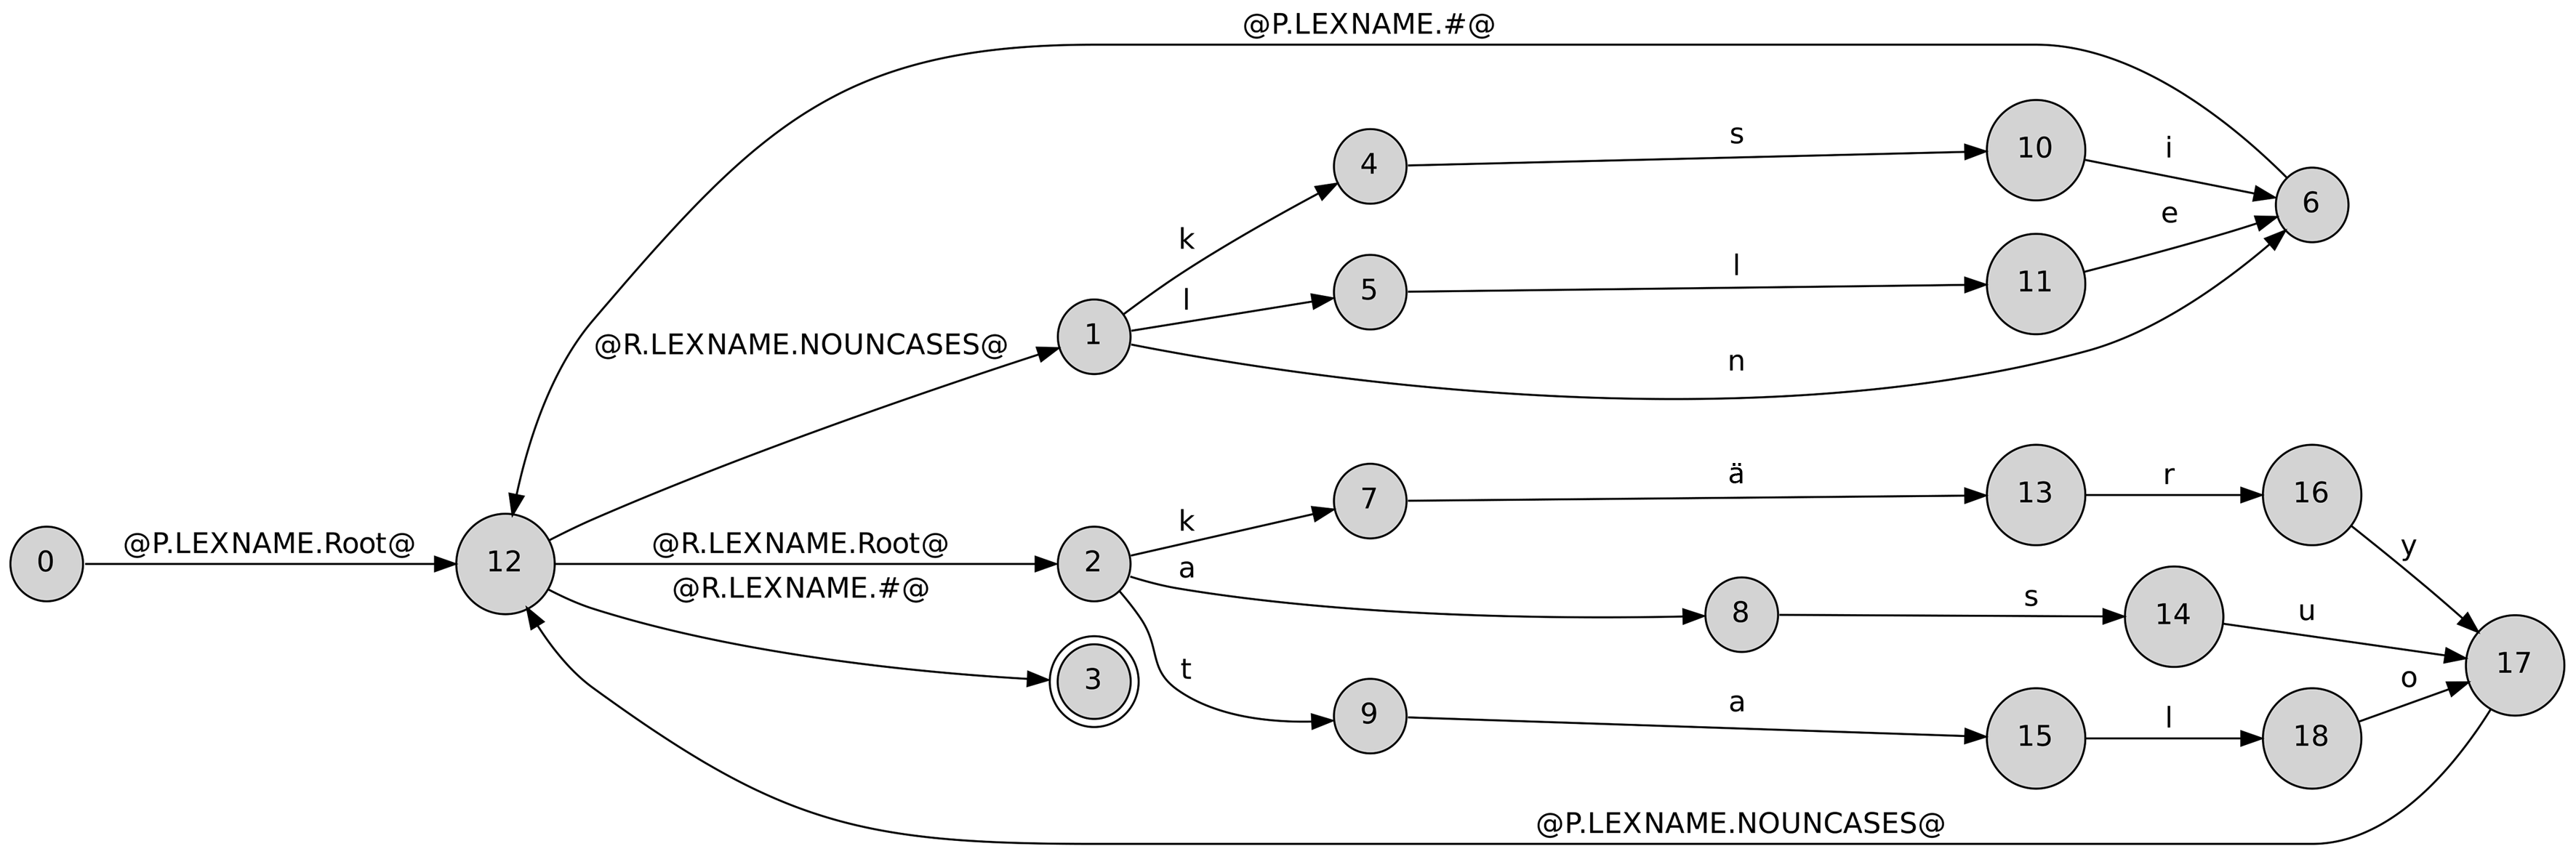
\includegraphics[width=\textwidth]{transducer.png}
     \caption{Simplified part of Finnish lexc grammar description with automatic flags
     \label{fig:lexc-fin-flag}}
\end{figure}

Additionally,
every morphological description starts with \texttt{Root}, which is
represented using the pair of flags
\verb+@P.LEXNAME.Root@@R.LEXNAME.Root@+ and ends with \texttt{\#}, which is represented using the pair of flags \verb+@P.LEXNAME.#@@R.LEXNAME.#@+.

The transducer built from the morphological description in
Figure~\ref{fig:lexc-fin} is shown in Figure~\ref{fig:lexc-fin-flag}.




% Second column
\newcolumn

\section{Removing flag-diacritics }
\justifying
Since real-world morphological descriptions may contain empty, or nearly
empty, continuation lexicons, inserting flags in those cases only
increase the size of the transducer, without gaining any
benefits. Therefore, those continuation lexicons need to be recognized and corresponding flag diacritics removed.
Additionally, rule composition with a flagged lexicon usually results in dramatical size
increase. In order to reduce the final transducer size, it is important to recognize which flag diacritics should be removed from the lexicon 
before composing it with rules.  

We have experimented with removing different flags and flags combinations from the lexical transducer 
to get an optimal transducer size after the composition with rules, the optimal results are shown in Table~\ref{table:sizes}. 


\section{Results}

\begin{table}[!h]
    \centering
    \begin{tabular}{|l|r|r|r|r|}
        \hline
        \bf Language & \bf Original & \bf With all flags & \bf After optimization & \bf \% \\
        \hline\hline
        \bf Greenlandic &   168 M  & 	185	M& 17 M & 10,1\%  \\
        \bf North Saami &   12 M   &  14 M	& 5,7 M & 47,5\%  \\
        \bf Finnish &   17 M     	 &	17 M 	& 16 M & 94,1\%  \\
        \bf Lule Saami  &   5 M    & 	19 M 	& 3 M & 60,0\%  \\
        \bf Erzya       &   3,7 M  &  16 M 	& 5,3 M& 143,2\%  \\
        \hline
    \end{tabular}
    \caption{Sizes of transducers without and with automatic flags (in megabytes); Percentage shows size of the flagged transducer after optimization, in comparison with the original
    \label{table:sizes}}
\end{table}

\justifying
In Table~\ref{table:sizes}, we show sizes of language transducers composed with grammar rules. First, there are sizes of original
transducers, then transducers compiled
with our new method that inserts all flag diacritics and finally flagged transducers after removing some of the flags. Look-up speeds, expressed in words per second, are shown in Table~\ref{table:lookup}.

\begin{table}[h]
 \centering
    \begin{tabular}{|l|r|r|r|}
        \hline
        \bf Language & \bf Original & \bf With flags & \bf \% \\
        \hline\hline
        \bf Greenlandic & 2 770 w/s & 2 507 w/s & 90,5\%  \\
        \bf North Saami & 30 714 w/s & 8 775 w/s & 28,6\%  \\
        \bf Finnish  & 84 415 w/s & 27 420 w/s & 32,5\%  \\

        \hline
    \end{tabular}
    \caption{Look-up speed of transducers without and with automatic flags; Percentage shows speed of the flagged transducer in comparison with the original
    \label{table:lookup}}
\end{table}



\section{Discussion}
\justifying
The results of this study show that large-scale language descriptions
can be compiled into smaller transducers using automatically inserted
flags. The effect is especially pronounced for language descriptions
which repeat morphemes in many different places, like the
morphological analyzer for Greenlandic. Since flag diacritics
themselves take space in the transducer graph, this method did not
offer improvements for descriptions where the original
transducer was small.

\section{Conclusion}

In this article we showed that by using morphologically motivated
flags we can dramatically improve the size of large lexical transducers. Automatically
inserted flag diacritics can make manual size optimization preformed by
linguists unnecessary, which may result in more readable and easier
to maintain linguistic descriptions.


\section{Acknowledgements}
\justifying
The research leading to these results has received funding from FIN-CLARIN, Langnet and the
European Commission's 7th Framework Program under grant agreement no. 238405 (CLARA).

\end{poster}
\end{document}